% AUTO-GENERATED by code/figlib.py helpers -- do not edit
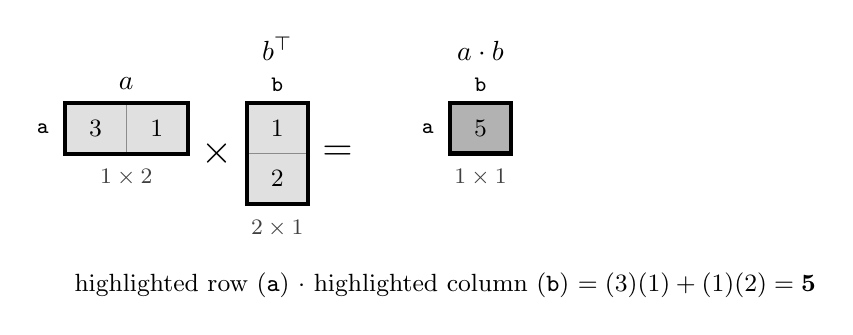
\begin{tikzpicture}
\draw[black!45, fill=black!12] (0.000,0.000) rectangle (0.780,-0.640);
\node[font=\small, text=black] at (0.390,-0.320) {$3$};
\draw[black!45, fill=black!12] (0.780,0.000) rectangle (1.560,-0.640);
\node[font=\small, text=black] at (1.170,-0.320) {$1$};
\draw[line width=1.4pt] (0.000,0.000) rectangle (1.560,-0.640);
\draw[line width=0.9pt] (0.000,0.000) rectangle (1.560,-0.640);
\node[anchor=east, font=\footnotesize\ttfamily] at (-0.080,-0.320) {a};
\node[anchor=south, font=\normalsize] at (0.780,0.050) {$\bm{a}$};
\node[anchor=north, font=\footnotesize, text=black!75] at (0.780,-0.720) {$1\times2$};
\draw[black!45, fill=black!12] (2.310,0.000) rectangle (3.090,-0.640);
\node[font=\small, text=black] at (2.700,-0.320) {$1$};
\draw[black!45, fill=black!12] (2.310,-0.640) rectangle (3.090,-1.279);
\node[font=\small, text=black] at (2.700,-0.959) {$2$};
\draw[line width=1.4pt] (2.310,0.000) rectangle (3.090,-1.279);
\draw[line width=0.9pt] (2.310,0.000) rectangle (3.090,-1.279);
\node[anchor=south, font=\footnotesize\ttfamily] at (2.700,0.020) {b};
\node[anchor=south, font=\normalsize] at (2.700,0.420) {$\bm{b}^{\top}$};
\node[anchor=north, font=\footnotesize, text=black!75] at (2.700,-1.359) {$2\times1$};
\draw[black!45, fill=black!30] (4.890,0.000) rectangle (5.670,-0.640);
\node[font=\small, text=black] at (5.280,-0.320) {$5$};
\draw[line width=1.6pt] (4.890,0.000) rectangle (5.670,-0.640);
\draw[line width=0.9pt] (4.890,0.000) rectangle (5.670,-0.640);
\node[anchor=east, font=\footnotesize\ttfamily] at (4.810,-0.320) {a};
\node[anchor=south, font=\footnotesize\ttfamily] at (5.280,0.020) {b};
\node[anchor=south, font=\normalsize] at (5.280,0.420) {$\bm{a}\cdot\bm{b}$};
\node[anchor=north, font=\footnotesize, text=black!75] at (5.280,-0.720) {$1\times1$};
\node[font=\Large] at (1.935,-0.640) {$\times$};
\node[font=\Large] at (3.465,-0.640) {$=$};
\node[anchor=north west, font=\small, align=left] at (0,-2.029) {highlighted row (\texttt{a}) $\cdot$ highlighted column (\texttt{b}) $= (3)(1) + (1)(2) = \mathbf{5}$};
\end{tikzpicture}
